\documentclass{article}
\usepackage{graphicx} % Required for inserting images

\title{Homework 5}
\author{Ayman Tawaalai}
\date{February 2024}

\begin{document}

\maketitle

\section{Introduction}
The purpose of the given assignment is to study and implement Hierarchical Clustering through practical means. The assignment states that the student must one hot encode and ngram the patient sequence data from homework 1. Once that is completed, it will serve as the input features of x. It will be used for clustering. Another task will be do the same clustering but with Principal Component Analysis (PCA).

\section{Hierarchical Clustering and PCA}
Hierarchical clustering is a machine learning model that creates a desired amount of clusters using trees. There are two different approaches, agglomerative, which takes a bottom up approach, and divisive, which takes a top down approach. The main benefit to use this model over K-Means is that it will be easier to recognize outliers.The main distance metric used to create a distance matrix of all the data points is euclidean distance. There are different types of linkages as well for the distance matrix. For example, single linkage will calculate for the smallest distance while avg will calculate for the average. The model will start off with many small clusters which will form together to create larger clusters. This will continue until there are no more clusters that could be merged or if there is a preset k that has been reached.

PCA is used to reduce the amount of dimensions in multi dimensional problems within a dataset. It uses basic concepts from Linear Algebra to accomplish this goal. The first step in PCA is to center the data around the mean for each feature. After a covariance matrix has been created using the mean centered data, the eigenvectors can be found and be ordered in descending order.

\section{Python Implementation}
The first task of the assignment is it conduct  Clustering analysis on the homework one data set. Loading the data, conducing one hot, and conducting PCA was done in a similar manner as was done in HW4. The distance matrix function works by taking in the one hot data and performing euclidean distance in a piece wise manner. After the distances have been calculated and placed in the matrix. The matrix is then resized to avoid duplicates within the matrix. For example, 2 to 3 and 3 to 2 will have the same distance. It is for that reason that loop occurs.
\begin{figure}
    \centering
    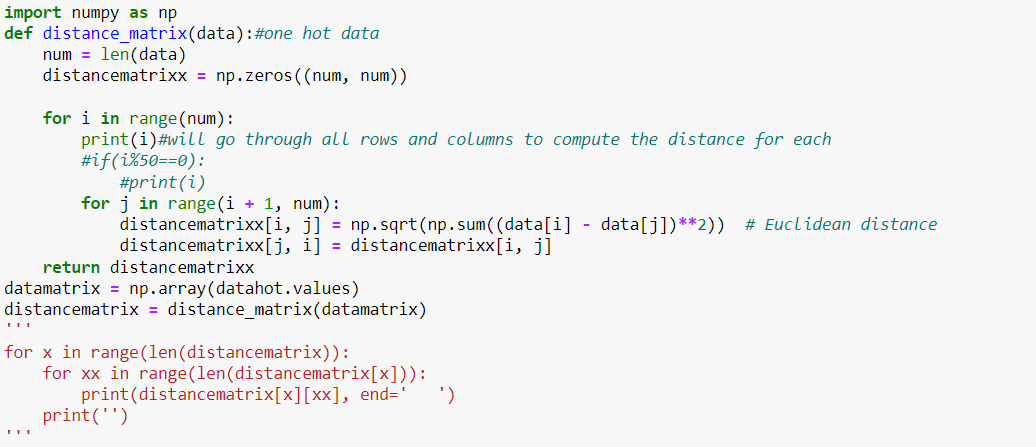
\includegraphics[width=0.5\linewidth]{a.png}
    \caption{Distance Matrix}
    \label{fig:enter-label}
\end{figure}
\begin{figure}
    \centering
    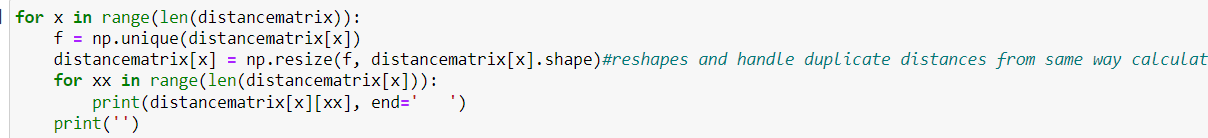
\includegraphics[width=0.5\linewidth]{b.png}
    \caption{Resize Loop}
    \label{fig:enter-label}
\end{figure}
The hierarchical clustering function will be that main work horse function for this model. It will continue calling functions that call other functions until the desired K amount of clusters have been reached. To make it easier, the distance matrix initializes itself into a dictionary and is returned into clusters. This is used to assist in merging and deleting clusters. The find closest clusters function will use single linkage to get the minimum distance for the closest cluster. One the work horse function is completed, it will return the final clusters back to the user and print it out.
The second outlined task is to incorporate PCA into this clustering model. The PCA steps are done in the PCA function. The function follows the outlined steps in section 2, Hierarchical Clustering and PCA, when it is called upon.
\begin{figure}
    \centering
    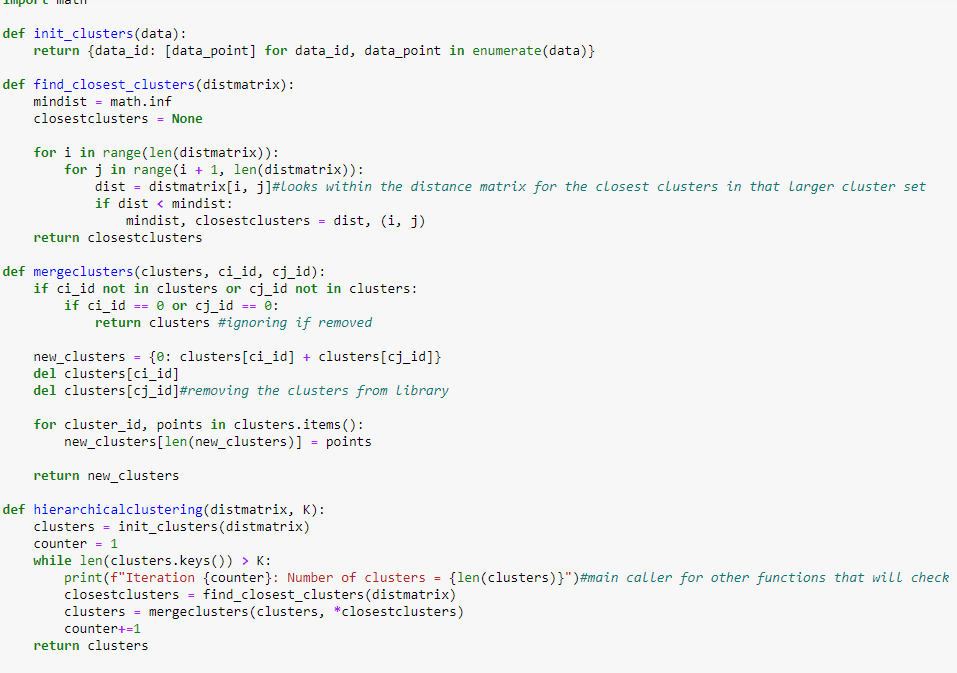
\includegraphics[width=0.5\linewidth]{c.png}
    \caption{Hierarchical Clustering python implementation}
    \label{fig:enter-label}
    
\end{figure}
\begin{figure}
    \centering
    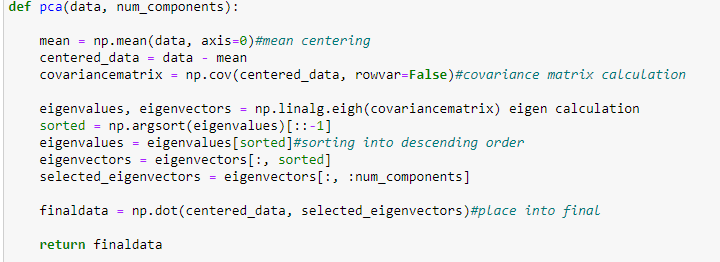
\includegraphics[width=0.5\linewidth]{d.png}
    \caption{PCA Function}
    \label{fig:enter-label}
\end{figure}
\section{WEKA}
There were many issues in trying to get WEKA to run the one hot encoded data. After many hours spent on trying to troubleshoot the issue, WEKA would repeatedly crash. This is because the patient dataset is too large to conduct hierarchical clustering within WEKA. 
\begin{figure}
    \centering
    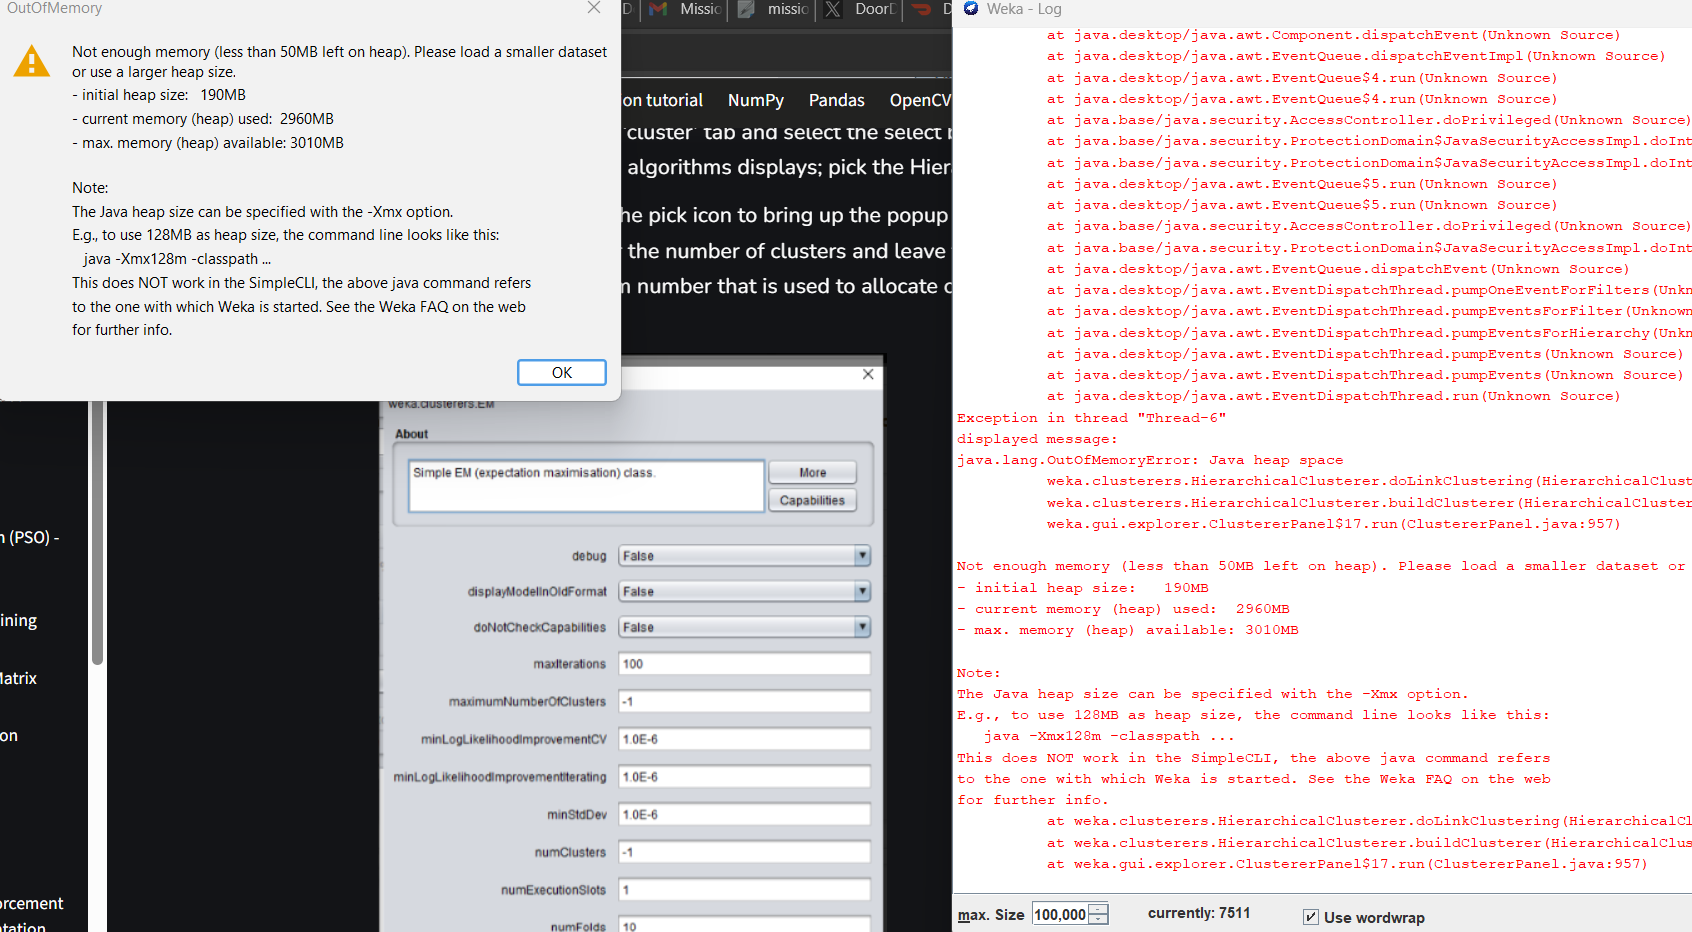
\includegraphics[width=0.5\linewidth]{e.png}
    \caption{WEKA Crash Log}
    \label{fig:enter-label}
\end{figure}
As a result, a smaller subset of the data had to be spliced to get it to run. The subset that will be used is the first patient data. The linkage used in WEKA will be single and it will calculate the distance using Euclidean. The result had all clusters reduced to one.
\begin{figure}
    \centering
    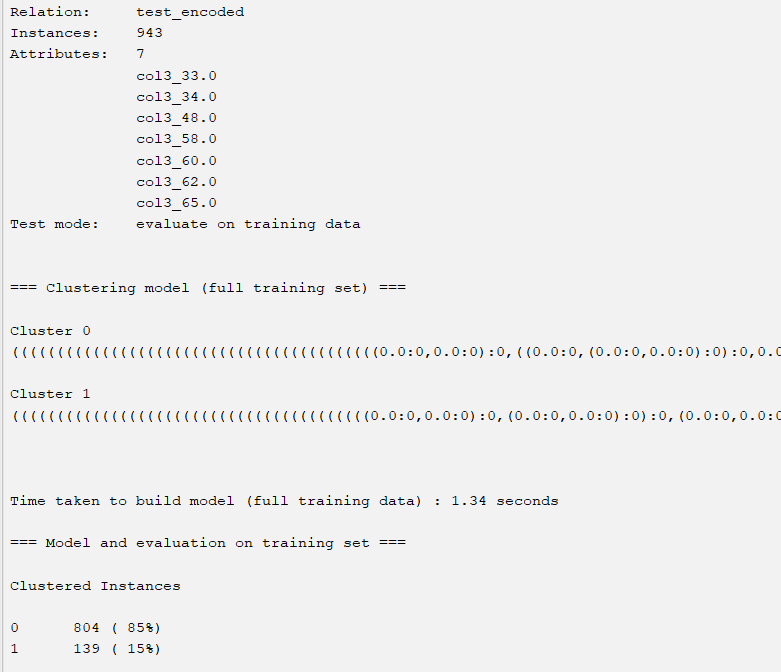
\includegraphics[width=0.5\linewidth]{f.png}
    \caption{WEKA output}
    \label{fig:enter-label}
\end{figure}
\section{Conclusion}
The purpose of the given assignment is to study and implement Hierarchical Clustering and PCA through practical means. The model proved to be highly accurate with the given data and handled outliers very well. However, because of its memory intensive operations it was very time consuming for the given dataset. In the future, it would be important for a machine learning engineer to chose which clustering algorithm it best based on how large the data set is.
\end{document}
